\section{\rqtwo: Do the Metrics Survive Measured Cost?}
\label{sec:rq2}

We now hold the metrics fixed and change one construct: the budget axis,
from sample count to measured acquisition cost
(Section~\ref{sec:costargument}).

\subsection{RQ2.1--2.2: Cost heterogeneity and the calibration of size as
a proxy}
\label{sec:rq21}

A fixed sample size is not a fixed measured effort. Within-system
per-configuration costs vary by up to a coefficient of variation of 1.42
and a $p90/p10$ ratio of 47.9 (BerkeleyDB-C) on the FSE artifact alone.
Consequently, the calibration ratio $\%cost/\%n$ of actual samples---1.0
when a sample is cost-representative---is centered near 1.0 in every
corpus but with heavy tails: 0.19--3.11 across FSE-artifact cells,
0.03--7.05 on ENERGY, 0.09--2.77 on WORKLOAD, 0.04--2.48 on LCBench,
0.64--2.57 on Linux, and 0.62--1.43 on x264
(Figure~\ref{fig:calibration}). In other words, sample size is an
approximately \emph{unbiased} but \emph{high-variance} proxy for
measurement effort: two strategies that both acquire $n$ configurations
can differ in actual spend by a factor of two to thirty, and the
direction of the deviation is strategy-systematic (e.g., \srs{} leans
expensive on Linux in 21/21 scopes, H6; \pilotcost{} leans cheap by
construction).

\begin{figure}[t]
  \centering
  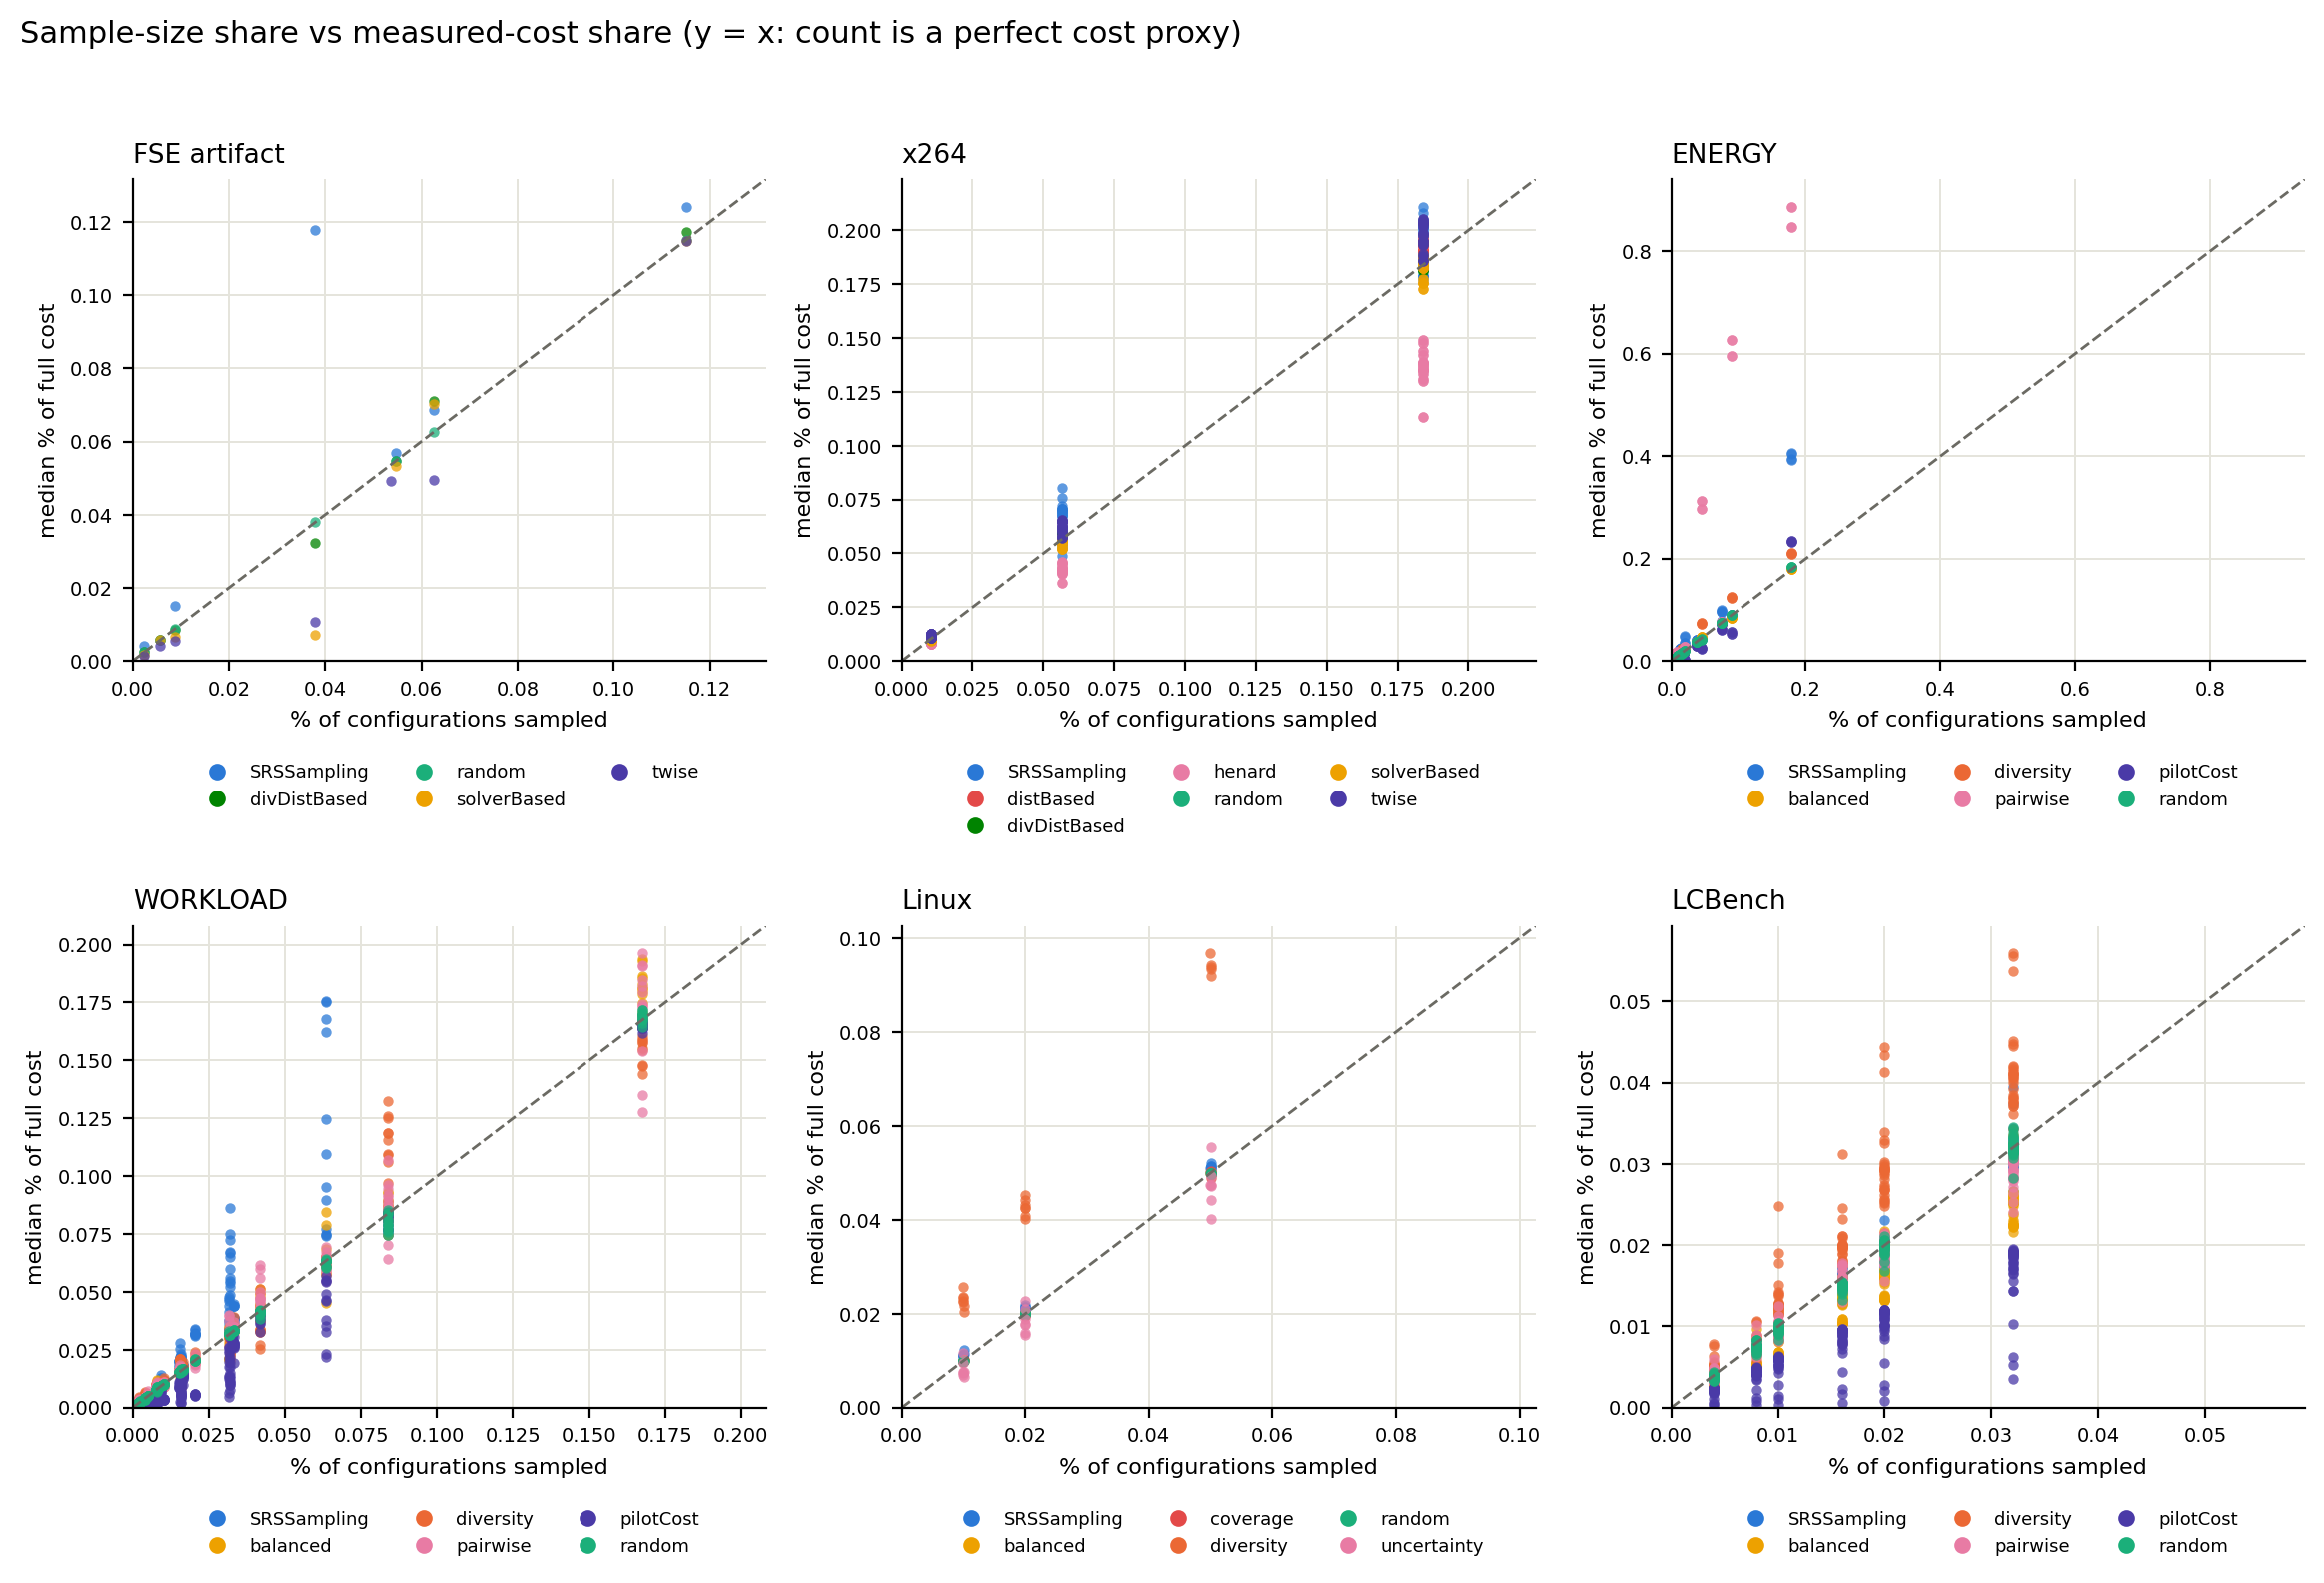
\includegraphics[width=.92\linewidth]{figures/fig_calibration_pct_n_vs_pct_cost.png}
  \caption{Share of configurations sampled versus share of total
  measurement cost, per strategy and budget level (medians across runs).
  On the $y{=}x$ diagonal, sample size is a perfect cost proxy.}
  \label{fig:calibration}
\end{figure}

\finding{Finding 5. Sample size is an unbiased but high-variance proxy
for acquisition cost: same-size samples differ in measured spend by up to
an order of magnitude, and the deviations are strategy-systematic---a
construct-validity gap for any budgeted strategy comparison.}

\subsection{RQ2.3: Decision impact}
\label{sec:rq23}

Does the proxy error matter for decisions? Two decision artifacts can
change when the budget axis switches from $n$ to measured cost: the
single top recommendation (highest $\omega$), and the Pareto frontier
over (integrated confidence, budget)---the set of non-dominated
(strategy, budget) choices a practitioner should consider.
Table~\ref{tab:impact} and Figure~\ref{fig:impact} give the counts.

\begin{table}[t]
  \centering\small
  \caption{\rqtwo{} decision impact per corpus: scopes where the top
  recommendation (H2) and the Pareto frontier (H4) differ between the
  size axis and the measured-cost axis.}
  \label{tab:impact}
  \begin{tabular}{@{}lrrr@{}}
    \toprule
    Corpus & Scopes & Top changes (H2) & Frontier changes (H4) \\
    \midrule
    FSE artifact & 7 & 2 (29\%) & 6 (86\%) \\
    x264 & 34 & 2 (6\%) & 30 (88\%) \\
    ENERGY & 220 & 31 (14\%) & 220 (100\%) \\
    WORKLOAD & 359 & 61 (17\%) & 346 (96\%) \\
    Linux & 21 & 13 (62\%) & 21 (100\%) \\
    LCBench & 210 & 120 (57\%) & 207 (99\%) \\
    \midrule
    Total & 851 & 229 (27\%) & \textbf{830 (97.5\%)} \\
    \bottomrule
  \end{tabular}
\end{table}

\begin{figure}[t]
  \centering
  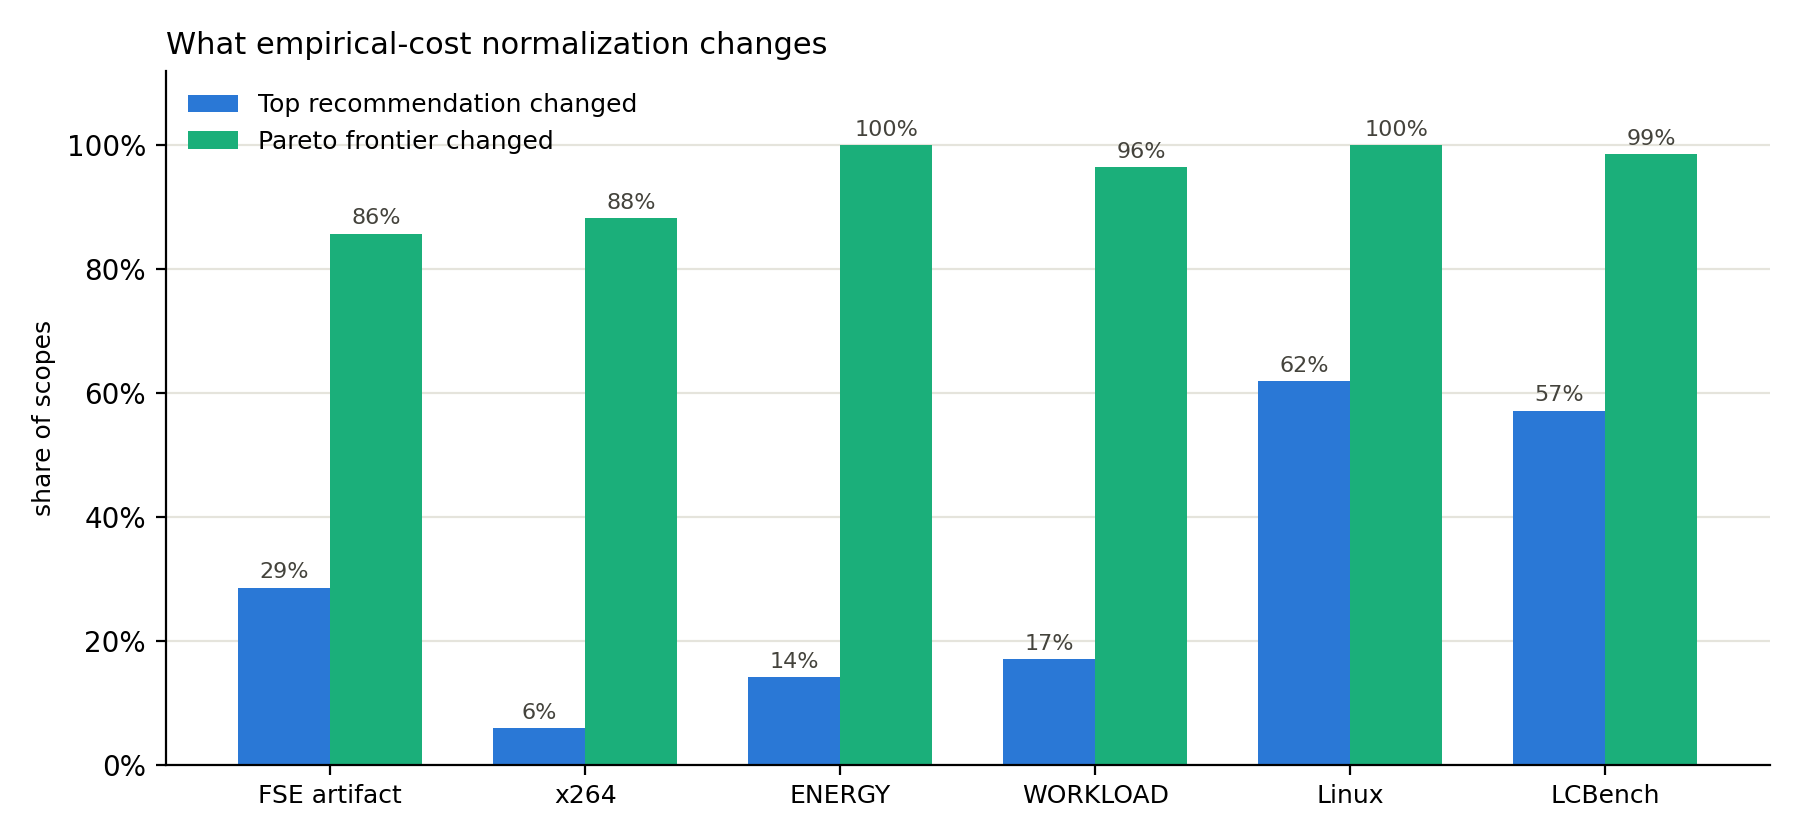
\includegraphics[width=.85\linewidth]{figures/fig_cost_normalization_impact.png}
  \caption{What switching the budget axis changes, per corpus: the single
  top recommendation versus the Pareto frontier of defensible choices.}
  \label{fig:impact}
\end{figure}

The frontier result is the most robust effect in our data: in 830 of 851
scopes (97.5\%), the set of guarantee/cost-efficient choices under
measured cost differs from the set under sample count, and not
marginally: the median Jaccard overlap between the two frontiers is
0.14--0.33 depending on the corpus. The top-1 recommendation is more
stable and strongly corpus-dependent---from 6\% of x264 contexts to 62\%
on Linux: the Pareto-level effect is the robust one, single-winner flips
the secondary one.

Even on the original FSE artifact, re-indexing by the artifact's own
runtime measurements changes the frontier in 6/7 systems.
Table~\ref{tab:fseartifact} gives the per-system view: cost
heterogeneity (columns 3--4) is a property of the system, and where it
is large (7z, BerkeleyDB-C), the size-indexed and cost-indexed winners
diverge---\srs{} wins both axes only on the three systems whose samples
happen to be nearly cost-representative. The frontier overlap (last
column) is below $0.5$ on six of seven systems.

\begin{table}[t]
  \centering\small
  \caption{Per-system decisions on the original FSE artifact at the $t2$
  budget. CV: coefficient of variation of per-configuration cost;
  $p90/p10$: cost dispersion; best by size/cost: winner by integrated
  confidence discrepancy under each budget axis; $J$: Jaccard overlap of
  the two Pareto frontiers.}
  \label{tab:fseartifact}
  \setlength{\tabcolsep}{4.5pt}
  \begin{tabular}{@{}lrrrllr@{}}
    \toprule
    System & $|\mathcal{V}|$ & Cost CV & $p90/p10$ & Best by size & Best by cost & $J$ \\
    \midrule
    7z & 68{,}640 & 1.19 & 10.1 & \srs & $t$-wise & 0.50 \\
    BerkeleyDB-C & 2{,}560 & 1.42 & 47.9 & \srs & \randomS & 0.20 \\
    Dune & 2{,}304 & 0.34 & 1.8 & \srs & \srs & 0.25 \\
    Hipacc & 13{,}485 & 0.44 & 2.6 & distance & distance & 0.25 \\
    JavaGC & 193{,}536 & 1.02 & 7.8 & \srs & \srs & 0.33 \\
    LLVM & 1{,}024 & 0.07 & 1.2 & distance & distance & 1.00 \\
    Polly & 60{,}000 & 0.24 & 2.1 & \srs & \srs & 0.20 \\
    \bottomrule
  \end{tabular}
\end{table}

\finding{Finding 6. Re-indexing guarantees by measured cost changes the
Pareto frontier of defensible (strategy, budget) choices in 97.5\% of 851
scopes---including 6/7 original FSE systems---while the single top pick
changes in 27\%. Sample-size budgets systematically misrepresent the
decision surface a cost-aware practitioner faces.}

\subsection{RQ2.4: Cost-normalized recommendation}
\label{sec:rq24}

Which strategy is best per unit of measured cost, by
$\omega_{\mathrm{cost}}$? Table~\ref{tab:winners} counts the
cost-normalized winners per corpus. \srs{} remains the winner where it
also won at fixed size---26/34 x264 contexts, 3/7 FSE-artifact
systems---but nowhere else: 9/220 ENERGY, 31/359 WORKLOAD, 0/21 Linux,
0/210 LCBench (Figure~\ref{fig:srsstatus}). On the small-budget families
the space-filling strategies dominate the cost-normalized picks
(\diShe{} 108 and \pairwise{} 74 of 220 on ENERGY; \pairwise{} 155 and
\diShe{} 108 of 359 on WORKLOAD), and on LCBench even the cost-aware
\pilotcost{} takes a quarter of the scopes (54/210)---a first hint of the
coupling mechanism that Section~\ref{sec:rq25} isolates.

\begin{table}[t]
  \centering\small
  \caption{RQ2.4, cost-normalized winners: how often each strategy has
  the highest integrated-confidence discrepancy against the cost-indexed
  prior ($\omega_{\mathrm{cost}}$), per corpus (winners with at least
  two scopes shown).}
  \label{tab:winners}
  \setlength{\tabcolsep}{5pt}
  \begin{tabular}{@{}lrl@{}}
    \toprule
    Corpus & Scopes & Cost-normalized winners (scopes won) \\
    \midrule
    FSE artifact & 7 & \srs{} (3), distance-based (2), $t$-wise (1), \randomS{} (1) \\
    x264 & 34 & \srs{} (26), Henard's (5), distance-based (3) \\
    ENERGY & 220 & \diShe{} (108), \pairwise{} (74), \balanced{} (20), \srs{} (9) \\
    WORKLOAD & 359 & \pairwise{} (155), \diShe{} (108), \balanced{} (48), \srs{} (31) \\
    Linux & 21 & \diShe{} (19), \textsf{uncertainty} (1), \balanced{} (1) \\
    LCBench & 210 & \diShe{} (69), \balanced{} (62), \pilotcost{} (54), \pairwise{} (25) \\
    \bottomrule
  \end{tabular}
\end{table}

Linux crystallizes the distinction between \emph{winning} and
\emph{being worth considering}. At full statistical power (100 seeds),
\srs{} is never the best cost-normalized strategy (0/21), its acquisition
cost differs significantly from random's in 21/21 scopes---it buys
systematically more expensive kernels---and yet it sits \emph{on} the
empirical guarantee/cost frontier in 19/21 scopes
(Figure~\ref{fig:frontiers} illustrates the three regimes: \srs{} best,
\srs{} on the frontier without winning, \srs{} dominated). \srs{} buys
real guarantee quality at a real cost premium; the cost-indexed analysis
does not dismiss the strategy, it \emph{prices} it.
Figure~\ref{fig:keysystems} shows two key extension systems in detail.
On the Linux~4.13 pool (92{,}562 kernels, 2\% budget level), \srs{} is
the archetypal frontier point: essentially the best confidence available
at its spend, while \diShe{} buys the final $5\cdot10^{-4}$ of
integrated confidence at more than twice the cost. On the lrzip energy
scenario, \srs{} is dominated---\diShe{} achieves more confidence at
half the spend---and the cost-aware \pilotcost{} is by far the cheapest
strategy yet delivers drastically weaker guarantees, previewing the
equal-spend mechanism of Section~\ref{sec:rq25}.

\begin{figure}[t]
  \centering
  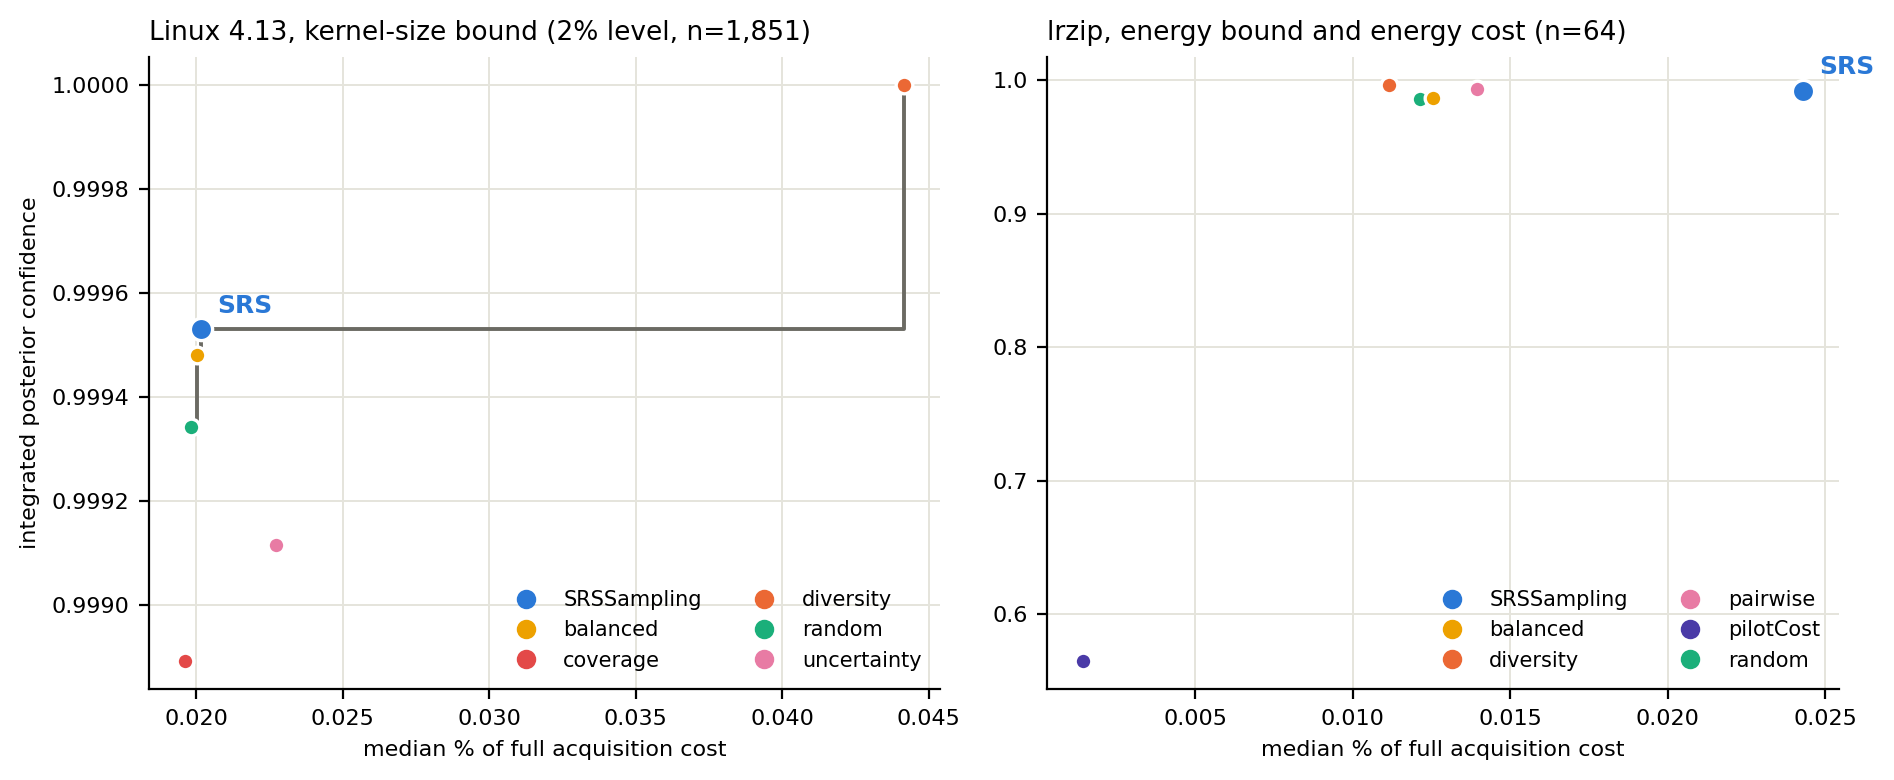
\includegraphics[width=\linewidth]{figures/fig_key_systems.png}
  \caption{Guarantee/cost view of two key extension systems at one
  budget level each (points: strategies; line: empirical cost/confidence
  Pareto frontier; median integrated confidence versus median share of
  full acquisition cost). Left: Linux~4.13, kernel-size bound
  (pool-relative; note the narrow confidence range). Right: lrzip with
  energy as both target and cost.}
  \label{fig:keysystems}
\end{figure}

\begin{figure}[t]
  \centering
  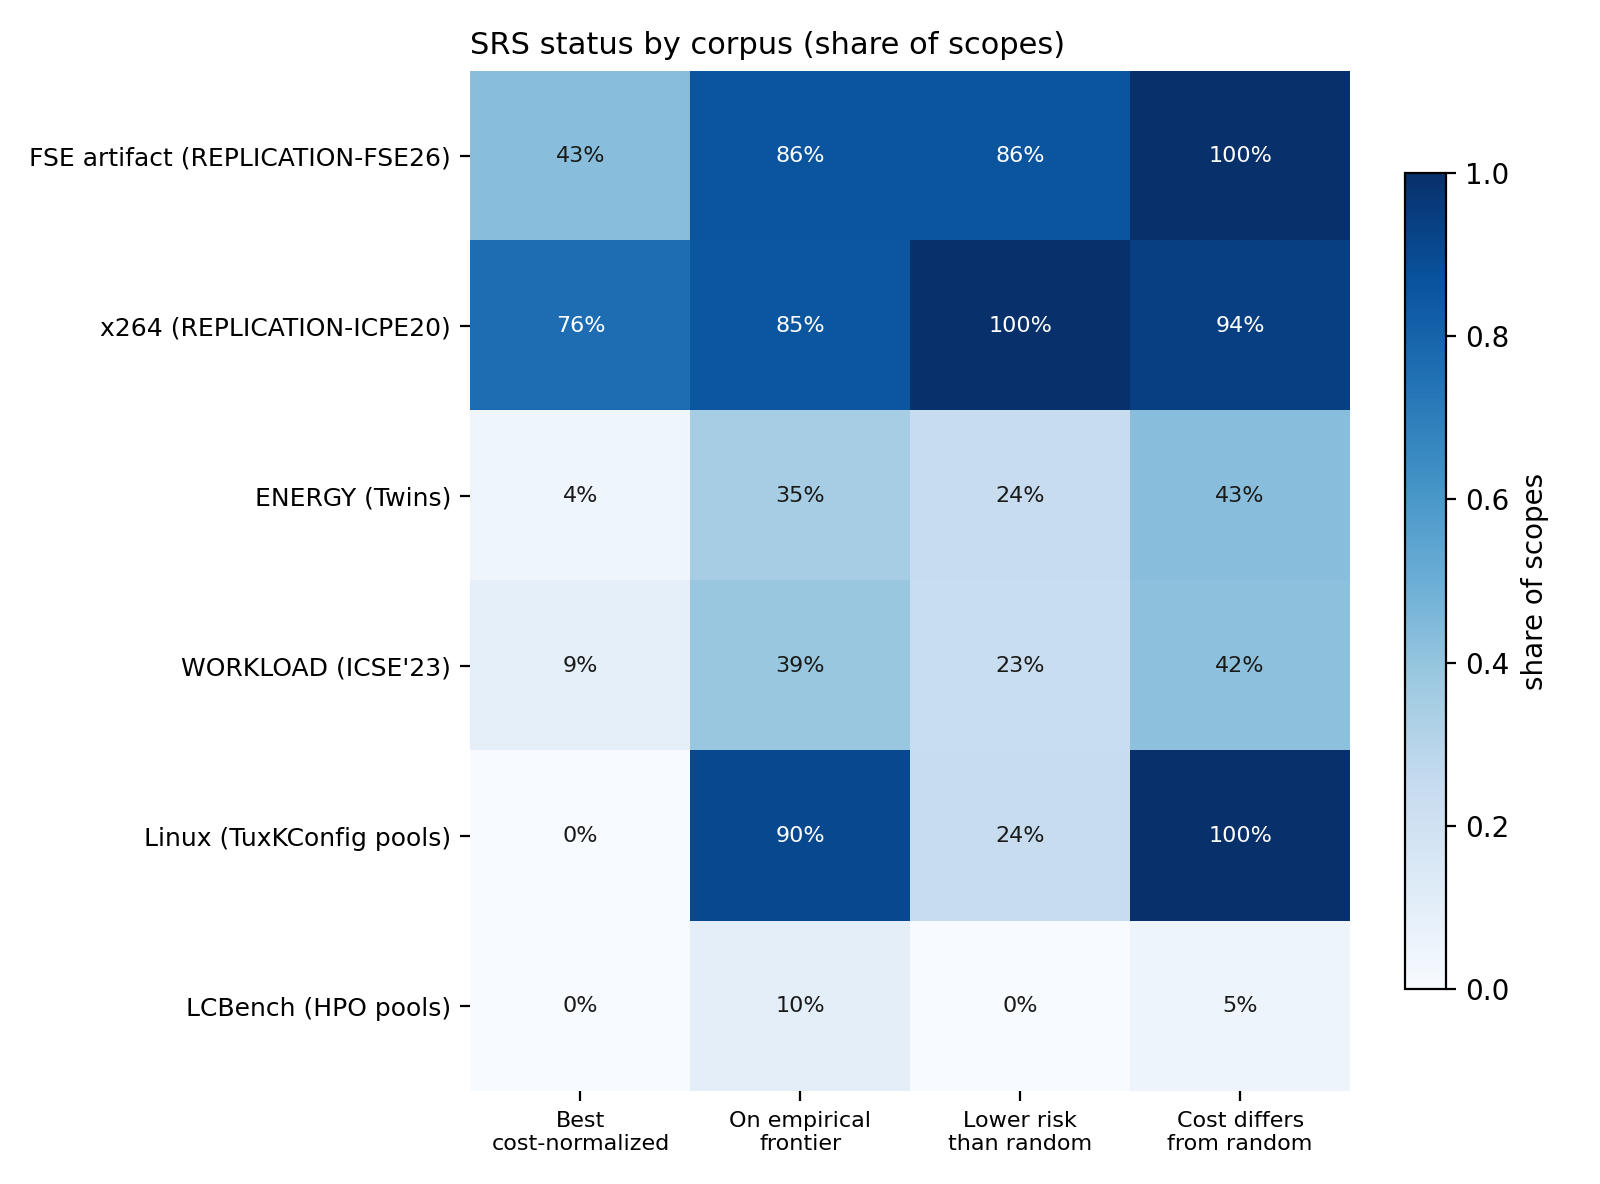
\includegraphics[width=.8\linewidth]{figures/fig_srs_status_matrix.png}
  \caption{\srs{} status per corpus under measured cost (share of
  scopes).}
  \label{fig:srsstatus}
\end{figure}

\begin{figure}[t]
  \centering
  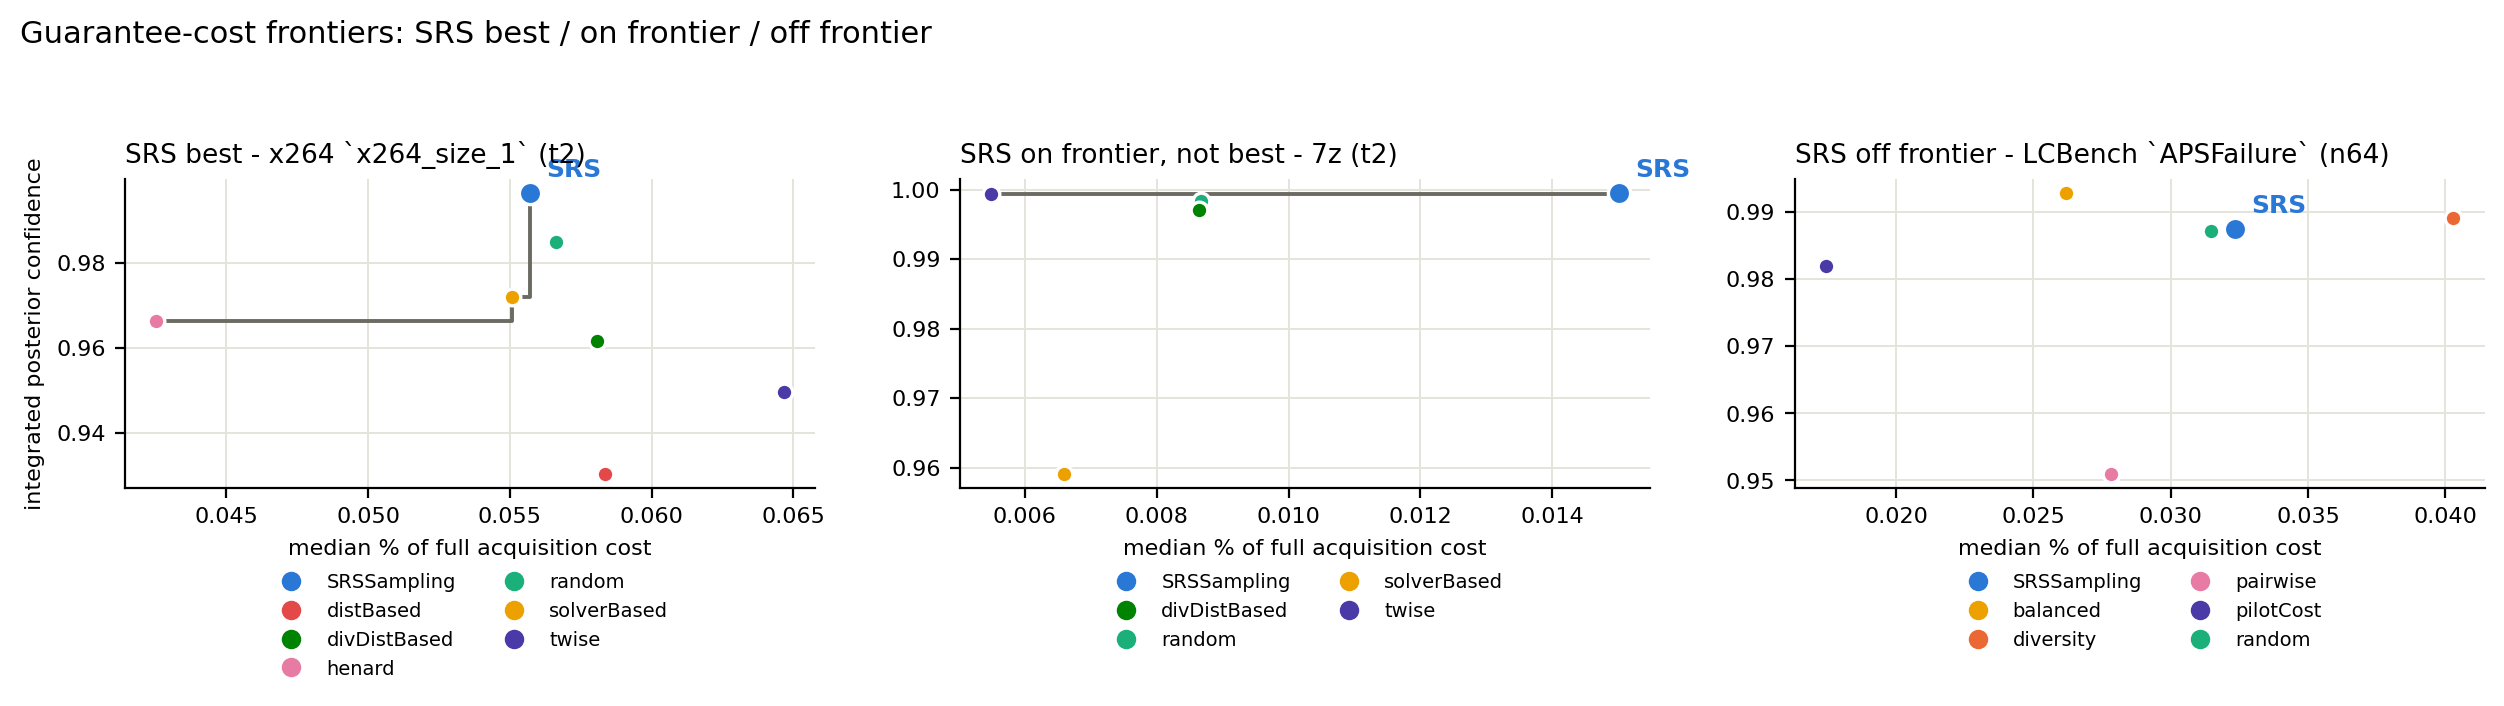
\includegraphics[width=\linewidth]{figures/fig_frontiers_representative.png}
  \caption{Representative guarantee/cost frontiers (points: strategies at
  one budget level; line: empirical cost/confidence Pareto frontier).
  Left: \srs{} best (x264). Middle: \srs{} on the frontier but not best
  (7z, FSE artifact). Right: \srs{} dominated (LCBench pool).}
  \label{fig:frontiers}
\end{figure}

\finding{Finding 7. Under cost normalization \srs{} keeps its crown only
on the replication corpora (x264 26/34; FSE artifact 3/7). On Linux it is
never best yet frontier-competitive in 90\% of scopes with an
always-significant cost premium: cost-indexing prices strategies rather
than dismissing them.}

\subsection{RQ2.5: Equal spend, and the mechanism}
\label{sec:rq25}

The $\omega_{\mathrm{cost}}$ handicap is a counterfactual. The
equal-spend protocol (Section~\ref{sec:equalspend}) makes it literal:
every strategy spends the same measured budget $B$ and buys however many
configurations $B$ affords. This is exactly the setting that cost-aware
strategy design targets \citep{sarkar2015cost,nair2017bad}, and
\pilotcost{} is built for it: it converts a fixed spend into
substantially more measured configurations than any cost-blind strategy.

\begin{figure}[t]
  \centering
  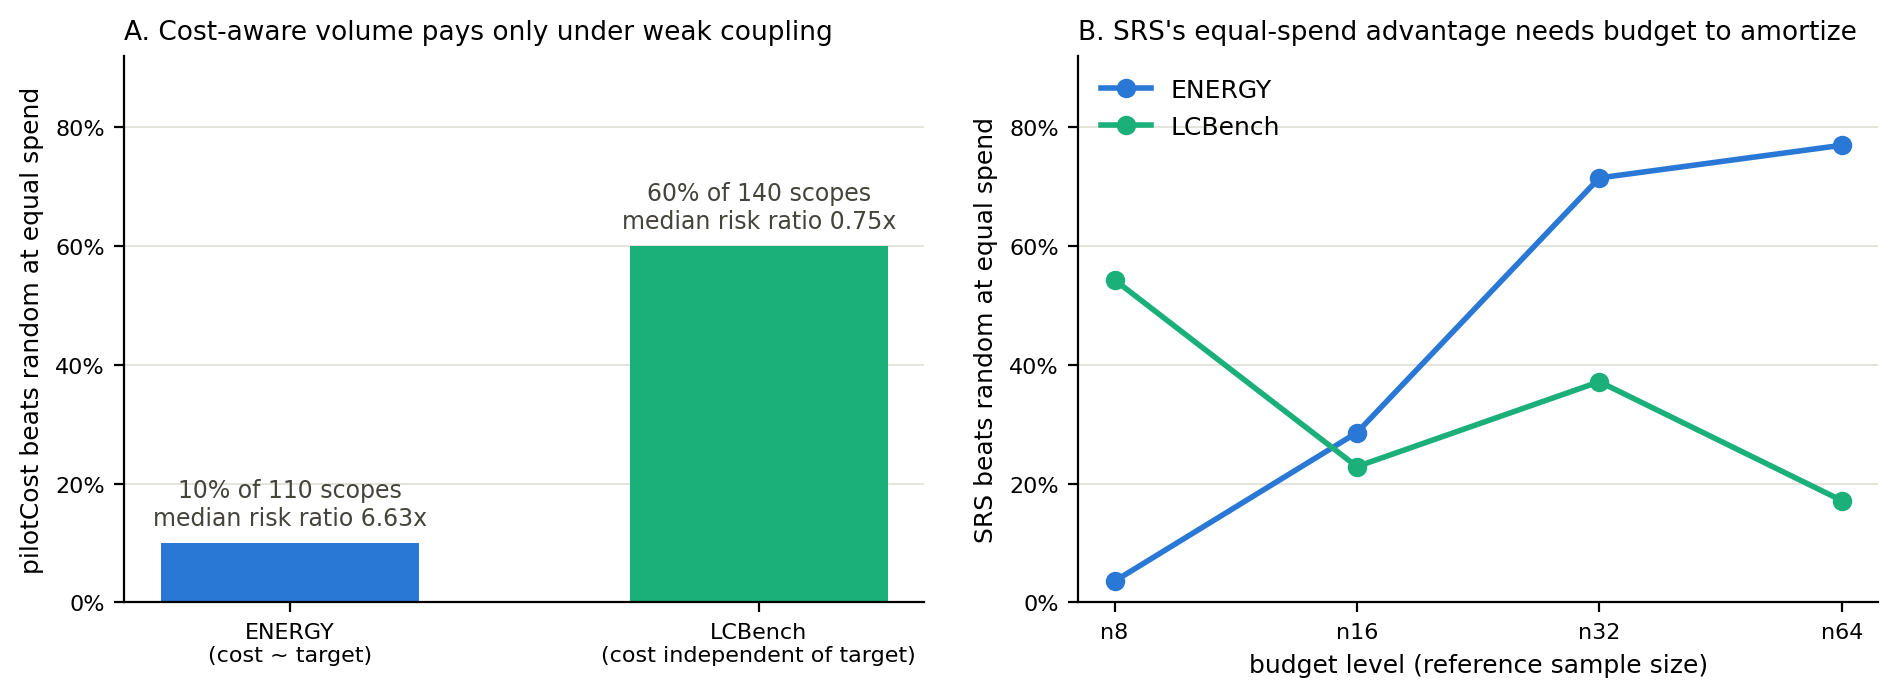
\includegraphics[width=\linewidth]{figures/fig_equal_spend.png}
  \caption{Equal-measured-spend experiments. (A)~\pilotcost{} versus
  uniform random across the coupling spectrum: share of scopes where
  \pilotcost's realized bound risk is lower, with the median risk ratio.
  (B)~Share of scopes where \srs{} beats random at equal spend, by budget
  level.}
  \label{fig:equalspend}
\end{figure}

For guarantees, the picture splits by \emph{cost--target coupling}
(Figure~\ref{fig:equalspend}A). On ENERGY, where cost (energy or
runtime) is strongly correlated with the bounded target, \pilotcost{}
converts its budget into $2.05\times$ more configurations (median; up to
$5\times$ on cost-heterogeneous systems)---and still loses: it beats
random in 11/110 scopes, with a median realized risk $6.6\times$
\emph{worse}. The information that a worst-case bound needs lives in the
expensive tail of the cost distribution, precisely the region a
cost-avoiding strategy refuses to buy; no volume of cheap configurations
substitutes for it. On LCBench, where training runtime and final accuracy
are only weakly coupled, the verdict flips: with a $1.66\times$ volume
advantage, \pilotcost{} beats random in 84/140 scopes with a median risk
ratio of 0.75. Cost-aware volume pays exactly when the outcome-relevant
information is \emph{not} concentrated in the expensive tail.

Table~\ref{tab:equalspend} summarizes both experiments.

\begin{table}[t]
  \centering\small
  \caption{RQ2.5, equal measured spend: every strategy buys the sample
  size the budget $B$ affords. Volume: \pilotcost's median affordable-$n$
  multiplier over \randomS. Risk ratio: median of
  \pilotcost's realized bound risk over \randomS's.}
  \label{tab:equalspend}
  \setlength{\tabcolsep}{4.5pt}
  \begin{tabular}{@{}lrrrrrl@{}}
    \toprule
    & & \multicolumn{3}{c}{\pilotcost{} vs.\ \randomS} & & \\
    \cmidrule(lr){3-5}
    Family & Scopes & volume & beats & risk ratio & \srs{} beats \randomS & Top winner \\
    \midrule
    ENERGY (cost $\sim$ target) & 110 & $2.05\times$ & 11 (10\%) & $6.6\times$ & 49 (45\%) & \diShe{} (47) \\
    LCBench (cost $\perp$ target) & 140 & $1.66\times$ & 84 (60\%) & $0.75\times$ & 46 (33\%) & \diShe{} (80) \\
    \bottomrule
  \end{tabular}
\end{table}

The same experiment resolves the \srs{} budget question raised in
\rqone{} (Figure~\ref{fig:equalspend}B). On ENERGY, \srs's equal-spend
win rate over random climbs from 1/28 scopes at $n8$-scale budgets to
20/26 at $n64$-scale: its recursive space restriction needs enough batches
to pay for itself, which is why it dominates at the original study's
$t$-wise-scale budgets and disappears at small ones. On LCBench the
gradient runs the other way (54\% down to 17\%): with cost and target
decoupled, random's cheap volume catches up with the pool's extremes
faster than \srs's guided-but-expensive search. Across both experiments
the overall winner is unchanged---\diShe{} wins 47/110 and 80/140
scopes---so the equal-spend protocol and the
$\omega_{\mathrm{cost}}$ handicap agree on every corpus-level conclusion,
ruling out the methodology as the explanation.

\finding{Finding 8. At literal equal spend, cost-effectiveness is
governed by cost--target coupling and budget amortization: the cost-aware
\pilotcost{} flips from $6.6\times$-worse to better-than-random as
coupling weakens, and \srs's advantage grows from 4\% to 77\% of scopes
as the budget grows. ``Cost-effective'' is a property of the (strategy,
outcome, coupling) triple---not of a strategy alone.}

\subsection{\rqtwo{} answer}

The FSE metrics themselves survive the re-indexing unchanged: posterior
risk, confidence, and $\omega$ are as computable and discriminative
against a cost-indexed baseline as against a size-indexed one. What does
not survive is the invariance of the \emph{decisions} they support. The
frontier of defensible choices moves in 97.5\% of scopes; the
cost-normalized winner is \srs{} only within the original population; and
equal-spend testing shows the governing mechanisms to be properties the
sample-size abstraction cannot express---where cost lives relative to the
target, and how much budget a strategy needs before its guidance
amortizes.
